\documentclass{project}
\usepackage[pdfauthor={M.J.Steel},pdftitle={Software Engineering Group Project, Maintenance Documentation},pdftex]{hyperref}
\usepackage[pdftex]{graphicx}
\usepackage{pdfpages}
\hypersetup{colorlinks=false,pdfborder={0 0 0}}
\begin{document}
\title{Software Development Life Cycle}
\subtitle{Maintenance Documentation}
\author{Mike Steel, Samuel Jackson}
\shorttitle{Maintenance Document}
\version{1.0}
\status{Finalised}
\date{2013-1-30}
\configref{SE.17.MN.01}
\maketitle
\tableofcontents
\newpage
\section{Introduction}
\subsection{Purpose of this Document}
This document is produced to aid an effective and sensible maintenance of the system produced previously as part of the System Development Life Cycle project, called Monster Mash. Herein are described all key parts of that system, the natures of them, and their usefulness to each other, including how and where data is stored, and why parts of the program are designed as they appear. \\
This document should be read and understood by anyone unfamiliar with the system before and changes are made by that person to any part.

\section{System Details for Maintenance}
\subsection{Program Description}
The Monster Mash Game is a web based program that, using a server side database and java methods, allows a user to create an online account and manage a list of monsters therein. A system of money allows the buying and selling and monsters, while breeding and battling allow users to interact and compete with each other. 

\subsection{Program Structure}
The program has three main levels of programming; the java, which handles the database and the main methods to manipulate that data for use in the game; the HTML and CSS, which creates the web page to display the program in, and is the entire user interface of the program; and lastly there is the javascript, which manages the interchange of data between the java controlling the database and the HTML and CSS controlling the user interface.

\subsubsection{Java}
The java is structured in a number of related classes that handle the data being requested from the database by the user, there are a number of different classes that each create a separate individual part of the game, including battling, breeding, and selling.

\paragraph{Battle.java}
Battle manages all battle related methods, it holds the following:\\
doBattle, which returns an arraylist of strings that are the victors of battles, is a short public method that calls the attack method and handles the entire battle round by round.\\
The next method is the private method declareWinner, used by the doBattle method to create an arraylist that holds a SQL statement to update the database. It updates the status of the winners and losers, and handles things such as setting health of the loser to 0, and adding victory money to the winner.\\
The final method in Battle.java is the attack method, which is a void method and uses variables atkMon and defMon to work out the amount of damage recieved by a monster from the given attacking monster's level and the defending monster's level.
\paragraph{Breed.java}
Breed.java is an enum class and contains the options SLIME, BEAST, DEMON, SERPENT, DRAGON, and GHOST.
\paragraph{Breeding.java}
Breeding.java handles the breeding of monsters and allows the creation of new monsters from the attributes of two parents.\\
There is only one method in this, which is doBreed, this takes the two users and their two monsters which are being bred, and from these calculates a new monster with new attributes based on the two previous monsters' attributes, a random amount is then added to this to give a chance of the new monster being more powerful than the previous two. An SQL statement is then generated and returned to the database to store the new monster.
\paragraph{Database.java}
The Database class manages the connection with the database, which allows the SQL statements generated by other classes within the program to be sent to the database. \\
The first method is the connect method; this creates the connection with the database.\\
createQuery is the next method and executes a query that another method of the java has generated previously, this then returns a ResultSet.\\
execute follows this method and takes a string, which is used to prepare an update statement for the database.\\
getConn is the penultimate method in this class and is used to get a connection variable.\\
setConn is the final mathod and opposite of the former, and is used to set a connection variable.
\paragraph{GameServer.java}
This class handles the management of connections between the server of the client, and actions that the client does that the server has to respond to.\\
The first method is called doGet and takes an Http Servlet request and response. This then works out whether the user is logged in, or whether user data has been requested by the user, depending on how the method is called.\\
The second is called IsLoggedIn, and takes a Http Servlet request and response, the same as the former method. It works out whether a user is logged in by finding out if their session has a username stored, if it is then the user is logged in, otherwise the user is not logged in.\\
Then there is GetUserData, which takes a HTTP Servlet request and response before printing the relevant articles returned to it and sending them on to the method from which it was previously called.\\
doPost is the next method and this again uses a Servlet request and response to get the kind of server interaction requested by the user; it is filled with case statements, which pick between a number of different options depending on the request sent to the server.\\
LogIn is the next method that allows a user to log into the server and manages a session with that user.\\
LogOut follows this and ends a session before setting a suer as logged out.\\
NewUser follows LogOut and is the method that handles the registration of new users, it creates the SQL queries to register them in the database and creates a new account with user name and password, as well as a new monster.\\
addFriend comes next and handles sending a friend request to another user for the to accept or decline.\\
newBattleRequest follows this and generates a new notification for a given user that a battle has been requested with them.\\
newBreedRequest is next and creates a new request for a given user to be accepted or declined.\\
newBuyRequest follows and handles a user buying another user's monster, it generates the SQL to handle money changes and monster transfers.\\
getMonsters comes next and gets monsters and their attributes.\\
getFriends gets a list of friends and their details.\\
getFriendsMonsters gets a list of friends and their monsters.\\
changeName allows a user to change the name of a given one of their monsters.\\
getAllResults gets the currently existing results of all battles that included the user who is requesting the data, and generates an SQL query to get this data.\\
getAllRequest is used on the notification page and is used to get all notifications that a user has.\\
acceptRequest is used to manage the acceptance of a request by a user who has received one. \\
acceptBattleRequest is used to accept a battle request by a user who has received one, and initiates a battle using Battle.java.\\
acceptFriendRequest is used to accept a friend request from the notification page and generates the SQL necessary to add that friend into the database.\\
declineRequest is used to remove a request without accepting it, and generates the necessary SQL for such an action.\\
setBreedCost is used on the auction page to set the breeding cost of a monster, and generates the SQL for that process.\\
setBuyCost does much the same as the previous function, except rather than setting a breed price it sets a price to sell the monster entirely.\\
getRichList is used on the friends page to your friends in order of richest to poorest, as well as display the amount of money that they have.\\
reloadfreinds is a method that reloads the friends that a user has and refreshes them, and generates the SQL necessary.\\
reloadmonsters does the same as the above, but for a list of your own monsters.\\
The final method in the class isreloadnotifications, and refreshes the notifications that a user has, also generating the SQL for it.\\
\paragraph{Monster.java}
This is used to manage the creation and life of monsters.
Firstly, monster has its own method also called Monster, which creates an instance of it with a name and an owner.\\
There are then two methods to handle the money that a monster sells for, one called getCashSell that gets what another user has set their monster to be sold for, and another called setCashSell that allows a user to set a sell value for a given monster.\\
Next there are two methods to handle the amount that it costs to breed with a monster, one called getCshBreed, which gets the amount that it costs to breed with a monster, and one called setCashBreed, which allows a user to set an amount that it will cost to breed with a monster.\\
Then there is generateStats, which generates the attributes of a new monster.\\
The above calls generateGenetics and generateBases, the latter generating base attributes of a monster, and the former generating a random amount to add or take away from that to create a unique set of stats.\\
There is also ageHealth and calculateAge, which relate to the ageing and status of the monster through its life.\\
\paragraph{MonsterStats.java}
Contains the same methods as the above class, except for the four relating to sell and breeding prices.
\paragraph{Request.java}
Request just sets up a number of variables for use as an instance of itself, and has no major functions that affect or put to use other methods or classes.
\paragraph{RequestState.java}
RequestState is an enum class that contains the states that a request can be in, these are ACCEPTED, VIEWING, PENDING, and DECLINED.
\paragraph{RequestType.java}
RequestType.java, like the above, is also an enum and contains the types of request there can be, including battling, breeding, and adding as a friend.
\paragraph{Status.java}
This again is an enum class and contains the different states that a monster can be in, it should be noted that they are not all implemented in the currently released version of this program, these options are NORMAL, SICK, DEAD, and HAPPY.
\paragraph{User.java}
User mainly sets up variables for the creations of instances of itself, it does contain the getMonster method which gets a list of all monsters that a user owns.
\paragraph{UserManager.java}
The first method in this class is fetchUserFromDatabase, which gets a user's details from the database by their ID, then there is another of the same name that fetches the data by Username.\\
Then there is cheakForUsersMonsterss, which checks whether a user has an existing monster.\\
This method is followed by generate, which generates a new monster if the user has none.\\
Then there is fetchMonsterFromDatabase, which takes the user ID and finds the monsters that that user has.\\
Following this is fetchFriendsMonstersFromDatabase, which finds all of the monsters that friends have and sends them to the user.\\
There are two fetchUser methods, one returns a username from a given name, the second returns a username from a given ID.\\
There are then two small methods to add and remove a user, as well as one to create an instance of a new user, and a final one to create a new request between two users, which takes the two users' IDs and their two monsters' IDs.

\subsubsection{HTML and CSS}The HTML bases all styles off of the stylesheet base.css, so all visual changes to the HTML style must be done through the CSS stylesheet. A number of parts of the HTML that the css affects are generated by the javascript, which fills a web page with the user's data that is then changed by the CSS into a more aesthetic style. These HTML tags are added in by the javascript, and so styling of these parts of the web page should be adapted via changes to the javascript files and the data that they output.

\paragraph{index.html}
There are many small html pages that simply contain the different titles for each page and are applied over the Index.html to create the appearance of individual pages. Therefore index.html is the key file and contains all of the parts as affected by the CSS file, the tabs and other parts are implemented here but any style changes should be made in base.css.

\paragraph{base.css}
This contains all of the different styles that are applied to the web site and any changes that need to be made to the look of the site should be implemented here.

\subsubsection{Javascript}
The Javascript is used in transactions of data between the client and the server; it validates data and conducts minor processes on that data before making sure that it is stored. Alternatively, it can conduct a process on the data within the database, before displaying it to the user by manipulating it into the correct HTML tags during web page generation.\\
\\
There is a javascript file relevant to each webpage that the user can visit within the monstermash site, each of these contains a number of methods that are then called and used within the particular page that they are relevant to. 

\paragraph{auction.js}
Auction.js contains getMonsters, which allows a user to see a list of all their monsters, tehre is also getFriends so that a user can see a list of all their friends. There is also getFriendsMonsters called so that a list of friends' monsters can be displayed. These are all added into the HTML code taht is generate by way of a number of functions that added on click events to names so that menus can be expanded.
\paragraph{base.js}
Base.js implements the logout and isLoggedIn functions from the java, useful on every page to check for or end sessions.
\paragraph{battle.js}
Battle.js implements sending data to and getting it from the getFriends, getFriendsMonsters, and getMonsters methods to create a list of friends and monsters that can battle and that you can choose to battle each other.

\paragraph{friends.js}
Friends.js implements the exchange of data using the getFriends and getRichList methods to create lists of friends and a way that you can see your friends organised by wealth. It then has built in outputFriendsList and outputRichList functions which display the returned data.

\paragraph{login.js}
There are two validation parts at the start of this file that validate both the login screen and the registration screen. There then follows a postLogin function, which directs user data to the server, a redirect function, which takes the user to the game if the login data is correct, and a validateUserDetails function that outputs a message if there is a problem with the validity of data input.

\paragraph{menu.js}
This is a currently unimplemented javascript file that was planned as a control file for the navigation menu.

\paragraph{notification.js}
This javascript file starts by getting data from the getAllNotifications method, allowing it to find all the notifications that a user has. This is followed by the addResponseEvents function that adds an on click option to each of these so that a user can accept, decline, or view certain notifications and their results. It then has the writeNotification function, which writes out the buttons relating to each function as well as the html to display the notifications themselves.

\paragraph{profile.js}
The profile page firstly uses the java method getUserData to get data about the user from the database, as well as the getMonsters java method to get the monsters owned by that user from the database. It also outputs a table of those monsters from the javascript function that accesses the method. It also creates the change name button for monsters by using the addChangeNameEvents, which is appended to each monster within the monsters table. There is then the buildProfileHTML function that creates the page and displays everything.

\paragraph{results.js}
The results.js file first uses the getAllResults java method to get any results left from battles or breeding that are within the database, there is also an addResponseEvents that handles hiding these results by pressing an OK button. There is the writeResult function, which begins writing the results page, this is then followed by the functions writebattleResult, writeBaby, and writeBuyResult, which manage writing out certain results to the page and formatting them respectively. The last function is writeResponse, which handles the result fading away after OK is pressed.

\paragraph{general.js}
Within the general.js file there is the getGETvars function that finds the functions that have been passed through Get to the URL, it then decodes the arguments and returns them. Following this there is the outputList function that outputs the HTML of a page, tyhen the getParentID, which gets the ID of an object that is selected. Following this there is an isint function for general use that parses ints from other variable types, a buildMonsterHTML function that builds a general table of monster details for use in the website, a buildFriendHTML function that does much the same but for friends, a verboseType function that turns a response from the server into a message readable by a user, and finally a generic server response function called writeServerResponse.

\paragraph{validate.js}
This is the final major javascript file and is used for validation on a number of parts of the website; there is the validateEmail function that takes an input and decides whether it is a valid email address, then there is the validatePassword function that validates whether a password is long enough to be a valid password, then lastly there is the validateNewPassword which does much the same as the previous function, but for a new user's password. 

\subsection{Algorithms}
\subsubsection{Registering a New User}
This sequence diagram shows a user accepting a battle request that has been sent to them by a friend. The diagram shows the users response being sent to the server using the doPost method. The request then runs through the relevant classes in order to gain the information required.\\
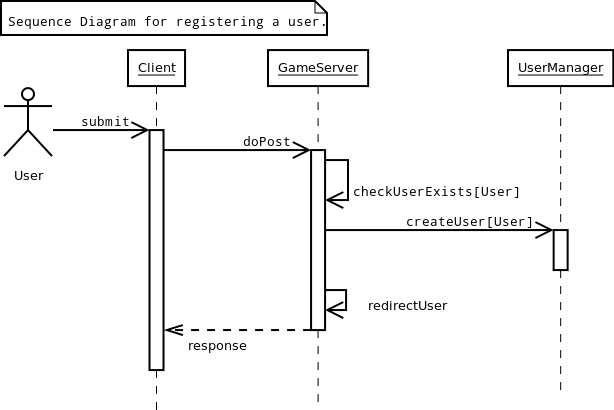
\includegraphics[scale=0.6]{SD_register_user.png}
\newpage
\subsubsection{Logging In}
This sequence diagram shows a user logging in to monstermash. The user submits their login information and it is posted to the server using the doPost� method. The request then runs the the relevant classes, checking the login details. A response is generated if the login details are invalid or the user is logged in if their details are valid.\\
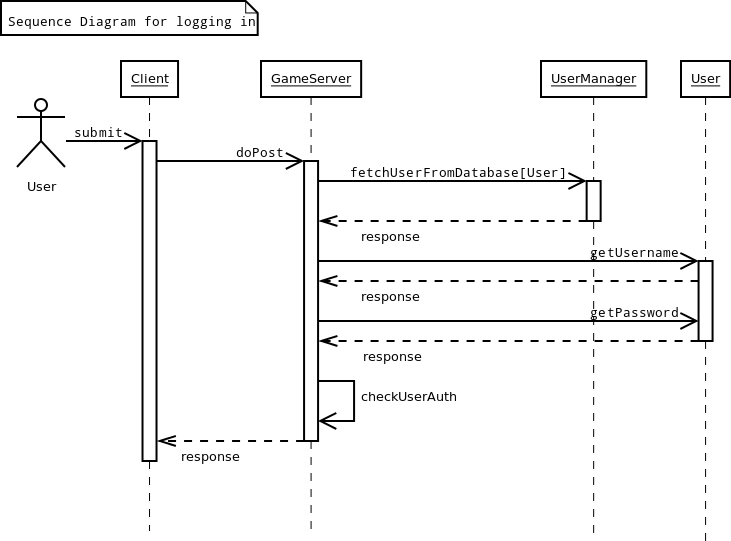
\includegraphics[scale=0.6]{SD_user_login.png}
\newpage
\subsubsection{Add Friend}
This sequence diagram shows a user adding a friend. The users request is sent to the server using the doPost� method. The request then runs through the relevant classes in order to gain the information required. A request is then sent to the corresponding user using the addRequest� methodad user class.\\
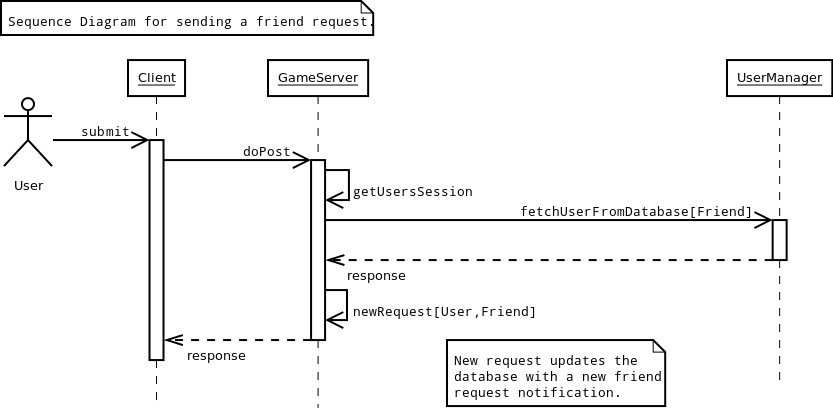
\includegraphics[scale=0.6]{SD_add_friend.png}
\newpage
\subsubsection{Sending a Battle/Breed Request}
This sequence diagram shows a user sending a breed or battle request to a friend. The diagram shows the users request being sent to the server using the doPost� method. A request is then sent to the corresponding user using the addRequest method and User class�.\\
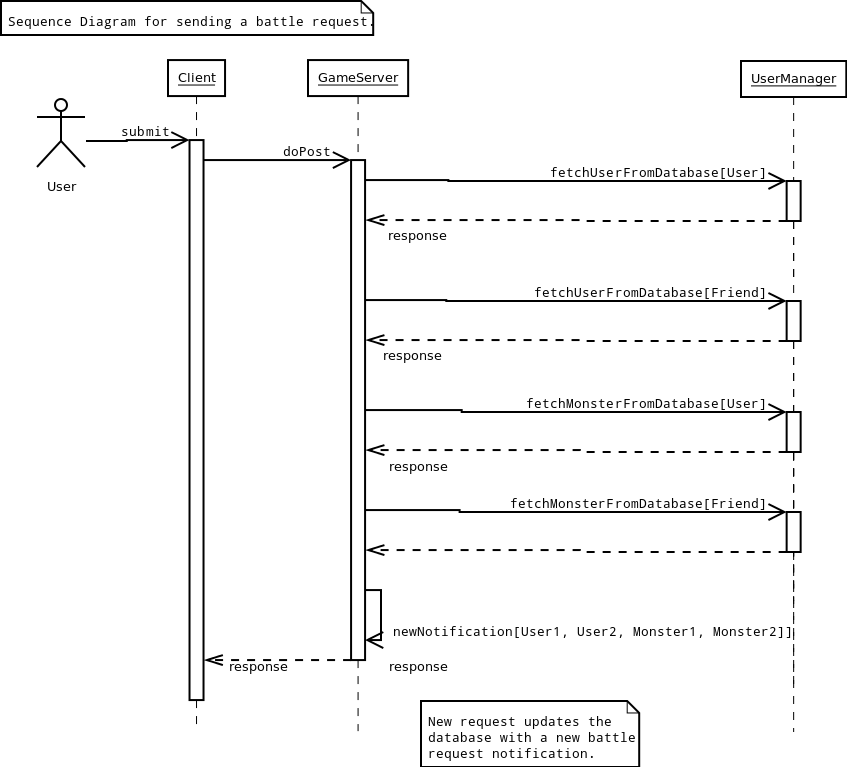
\includegraphics[scale=0.6]{SD_request_battle.png}
\newpage
\subsubsection{Accept Breeding}
This sequence diagram shows a user accepting a breed request that has been sent to them by a friend. The diagram shows the users response being sent to the server using the doPost� method. The request then runs through the relevant classes in order to gain the information required.\\
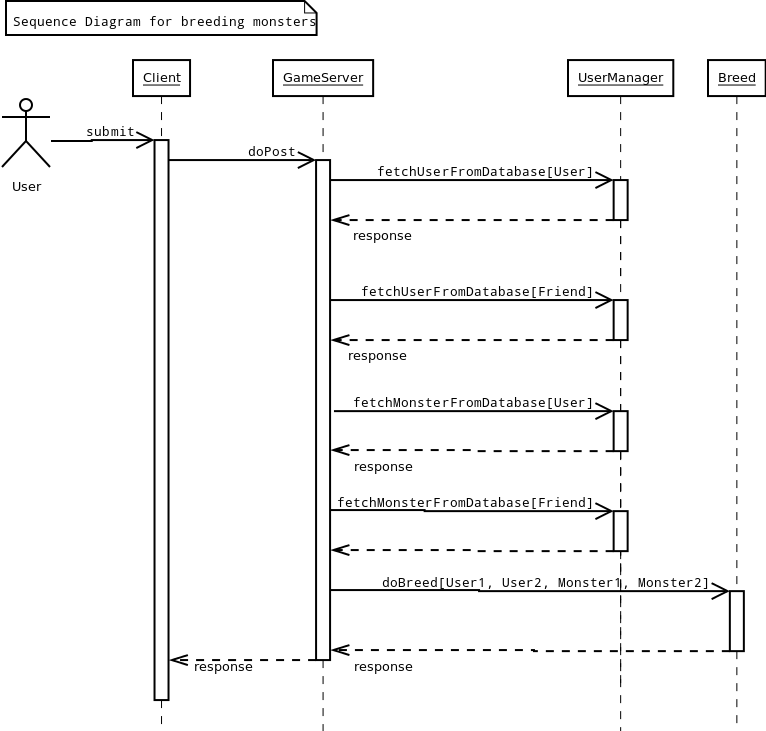
\includegraphics[scale=0.6]{SD_accept_breed.png}
\newpage
\subsubsection{Accept Battling}
This sequence diagram shows a user accepting a battle request that has been sent to them by a friend. The diagram shows the users response being sent to the server using the doPost� method. The request then runs through the relevant classes in order to gain the information required.\\
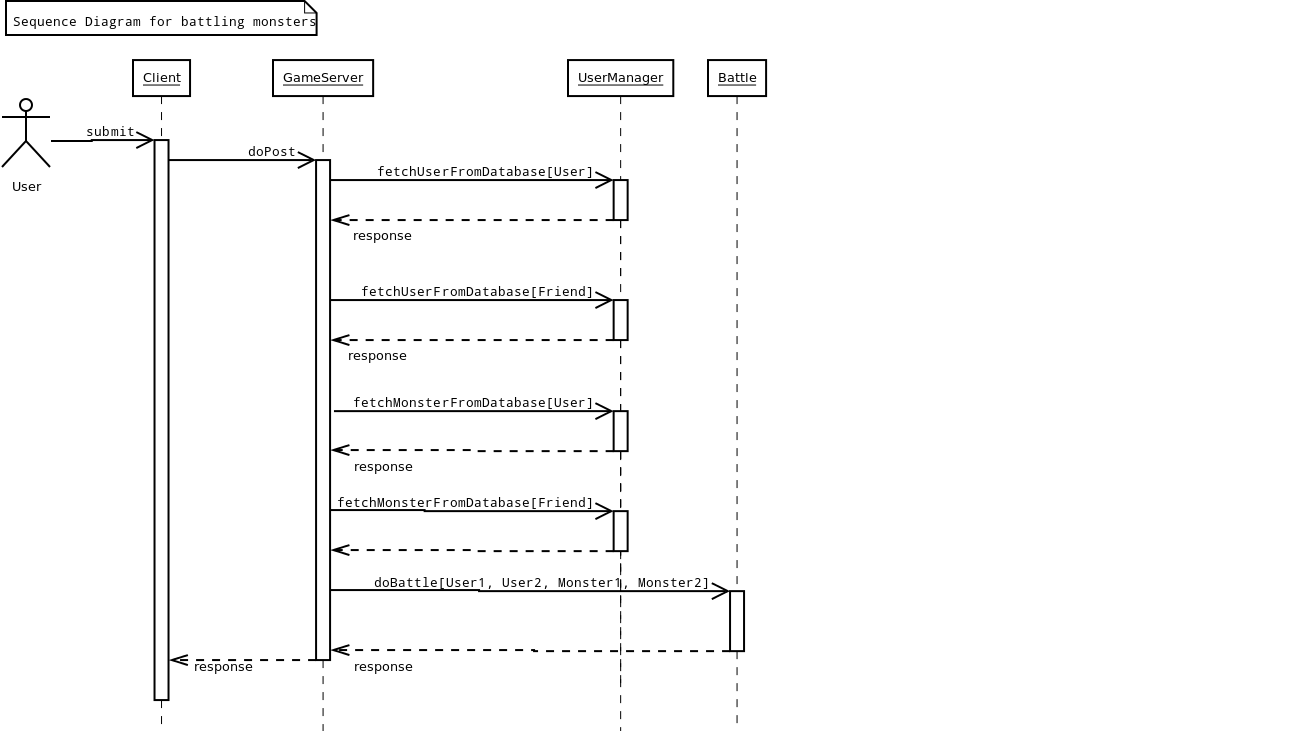
\includegraphics[scale=0.6]{SD_accept_battle.png}
\newpage
\subsection{Main Data Areas}
The main data storage facility of the Monster Mash program is in a database hosted on the server and accessed and manipulated by Java and Javascript. The user enters data on the client side of the website and this is then passed by the javascript into a number of java classes where the data is manipulated and put into SQL statements, from which it is placed into the database.

A few areas of larger data to note within the database, and possible causes of overload on the server at some point in the future, is that every player can have between one and an infinite number of monsters, meaning that there will always be much more monster data stored for monsters than for users, which may fill the database up at some point in future use of the program.
\subsection{Files}
User and monster data is only ever kept in the database. During client to server communication there is a session stored in a cookie on the client's computer, so if cookies are disabled this may not function correctly. Otherwise the only other files kept on the server are files that the program runs off, mentioned in the Program Structure section above.

The fact that the program relies heavily on javascript means that javascript will also have to be enabled on a client's browser, since without this the webpage will simply fail to display. However, since javascript and cookies are enabled by default on a browser, this shouldn't be a major hindrance for the program.
\subsection{Interfaces}
Although not directly controlled or influenced by any specialist input devices, the program does require standard hardware that any common computer should be associated with. The program will output to a client's monitor and require inputs from a keyboard, and a mouse is recommended for optimum use - but on-screen buttons can be tabbed between using a keyboard if a user would rather. Since most web-pages allow printing, the a printer would be an extra possibility for an output device if a user wanted to print out the screen and keep it for reference or other uses.

\subsection{Suggested Improvements}
\subsubsection{Unimplemented Functionality}
There are two functional parts of this program that were not implemented from the original specification, this was more down to the network problems that occurred over coding week than to any particular difficulty encountered in the coding of any of those parts. The first of these is monster ageing, which should age monsters over their lifespan and change their attributes as necessary, before killing them when they become too old.

The second functionality that the program is missing from the original specification is inter-server communication, however we had already organised a protocol with a number of other groups. Therefore, all that is missing is for us to produce the necessary code to allow our server to send data over to theirs, and thus would only take time to write the code, since methods of how the interaction would take place have already been planned.
\subsubsection{Added Functionality}
The program, as it stands, has a number of unimplemented java enums that appear in the code but are unused outside of their own declaration. These enums are things such as monster types, for example dragons or ghosts, and monster statuses, such as ill, which are as yet unused in the program. By implementing these it could add extra options for a user to have to deal with; such as creating random diseases that monsters can catch and user having to buy cures or risking the infection spreading. The unimplemented monster types could be used to add in things such as special attacks that are unique to monster types, or could split up different species of monsters and determine specific monsters that can only breed with other monsters of that type.

\subsubsection{Security and Usability}
There are a number of security flaws within the program at the moment, as well as a number of weaknesses that threaten the entire strength of the program as a functional system. The first of these is that the program is not entirely secure against SQL injections, and some javascript should be written to protect all input boxes from random SQL attacks; this can be done by parsing everything that is entered by javascript, both on the client side and on the server side, to check that it does not contain any series of characters that are dangerous.

Secondly, the program currently allows any user to have an infinite number of monsters, meaning that the database could fill up very quickly if even a small number of users started generating hundreds of monsters each. A method could be implemented to limit the number of monsters that any one user can have, although if the ageing process is implemented as recommended above then this should also hamper the amount of monsters that one user can have.

The third problem, though not an issue to the website or server's integrity, is an issue to usability, and this is the fact that the website will not run if either cookies or javascript are disabled. To make the website more usable then, a good addition would be some kind of message on the log in screen that is only shown when javascript fails or if the server cannot put a test cookie on the client's machine, this message would warn the user to enable javascript and cookies on their browser for optimum experience of the game.

Finally, the website is currently developed to run best in chrome, this is due to chrome being the most up to date and forward thinking browser, however, with so many people using other browsers, it would be an added advantage to have the same functionality in other browsers as is currently found in chrome.
\subsubsection{Design Additions}
The website has been implemented with an enticing css style to give a professional look and feel to the website to attract more users, but aside from this the design is still quite basic. A future development on this would be the implementation of images for different monsters, as well as the user perhaps being able to upload their own profile images. A custom font could also be implemented to replace to current fairly boring looking font.

\subsection{Possible Effects Caused by Change}
When making any additions to this program checks should be made to make sure that the correct SQL connections are maintained, and that the database and any cookies are still correctly accessed. It should also be made sure that javascript is still called from the correct files. So long as the current basis of the program is built on sensibly, with useful classes in java or javascript integrating with the current infrastructure, the program should continue to function correctly and be easy to maintain during future development and usage.

\subsection{Program Limitations}
The program is limited partly by the strength of the server, which may be overloaded if there is too much data being transferred at any one time, this could be improved by hosting the system on a more versatile server. The database also may use up a lot of memory if there are a lot of users registered with many monsters each, this could be corrected by hosting the database on a larger server, or by implementing a system of limiting monsters for each player, as well as having some system of clearing out data that has not been accessed in a while; i.e. delete inactive accounts that are taking up space on the server.

The client-side will also have limitations depending on their internet speed, their processing speed will also limit the program some small amount, but will not cause enough trouble to severely hinder the program, since the program itself largely runs on the server and only runs small amounts of javascript on the client side. The program will also be dangerously limited, if not stopped entirely, if the user disables cookies or javascript on their machine, so these should be enabled for the entirety of a client's use of the website. Since the javascript and cookies are not used to maintain any permanent data (which is instead kept in the website's database) deleting cookies between visits to the website will do no damage to a user's account, nor will it interfere with the website's functionality.

\subsection{Rebuilding and Testing}
The testing report and testing documentation included with this project should be apt to test the project thoroughly after any changes are made to any part of the system. Additional tests should be added to cover any new functionality implemented in the future. Testing guidelines are included in the final testing report as to how the testing was resolved for this project version and how it should be carried out in any future implementation of this system to ensure a complete and soundly working program.

\addcontentsline{toc}{section}{DOCUMENT HISTORY}
\section*{DOCUMENT HISTORY}
\begin{tabular}{|l | l | l | l | l |}
\hline
Version & CCF No. & Date & Changes made to Document & Changed by \\
\hline
1.0 & N/A & 2013-1-30 & Initial creation & MIS28 \\
\hline
\end{tabular}
\label{thelastpage}
\end{document}

